\chapter{Analysis formation, event selection and corrections}
\label{ch:analysis}

With the complete reconstruction of events in both data and simulation it is possible to begin forming an analysis.
Several variables are defined to be measured and an appropriate event selection must be formed, dependent on the event topology that is being investigated.
Corrections still need to be applied to the analysis objects to resolve any remaining differences between data and simulation.
Before the event selection, data objects are corrected depending on the response of the subcomponents in the detector, \eg{} there should be no angular dependence on the energy of a particle.
Then the simulation is then corrected to match what is observed in the data, \eg{} due to differences in the efficiencies of the various reconstruction algorithms applied.
Once the \ttbar{} yields have been calculated after all corrections are applied, then the cross sections can be measured.

\section{Kinematic event variables and the event selection}
\label{sec:var}
As stated in Sec.~\ref{sub:top_quark_cross_section_measurements}, this thesis measures seven event variables which are \NJET{}, \HT{}, \ST{}, \ptmiss{}, \WPT{}, \LPT{} and \LETA{}.
They are defined in the following way:
\begin{itemize}
	\item \NJET{} is the total multiplicity of jets in the event with $\pt>30\GeV$ and $\LETA<2.4$.
	\item \HT{} is the scalar sum of the \pt{} of these jets.
	\item \ptmiss{} is defined as the magnitude of the missing transverse momentum \ptmissvec{}, as defined in Sec.~\ref{sub:pf_ptmiss}.
	\item \LPT{} is the magnitude of the transverse momentum of the signal lepton.
	\item \LETA{} is the magnitude of the pseudorapidity of the signal lepton.
	\item \ST{} is the sum of the \HT{}, \LPT{} and \ptmiss{} event variables.
	\item {\WPT{} is the magnitude of the transverse momentum of the leptonically decaying boson defined as \\
	\begin{equation*}
		\WPT = \sqrt{(p^{\ell}_{x}+p^{\mathrm{miss}}_{x})^2+(p^{\ell}_{y}+p^{\mathrm{miss}}_{y})^2}.
	\end{equation*}
}
\end{itemize}

The event selection is performed using the collections of particles created following the methods described in Sec.~\ref{sec:analysis_objects}.
The signal event selection requires a single isolated tight lepton, either electron or muon, with zero additional veto leptons.
A minimum of four jets is needed, with at least two being tagged as coming from a \bquark{} quark.
% section event_selection (end)


\section{Jet energy corrections} % (fold)
\label{sub:jet_energy_corrections}

The response from the detector calorimeters to particles is not linear which means that a simple translation between reconstructed jet energy and particle-level jet energy is not feasible.
Jet energy corrections (\acrshort{jec}s) are used to provide the mapping between the measured and particle-level jet energies.
The \acrshort{jec}s are applied sequentially with each step correcting the jet energy scale (\acrshort{jes}) according to the associated jet parameters (\pt{}, $\eta$, flavour, \etc{}).
These steps are shown in Fig.~\ref{fig:JESFlow}.
\begin{figure}[htpb]
	\centering
	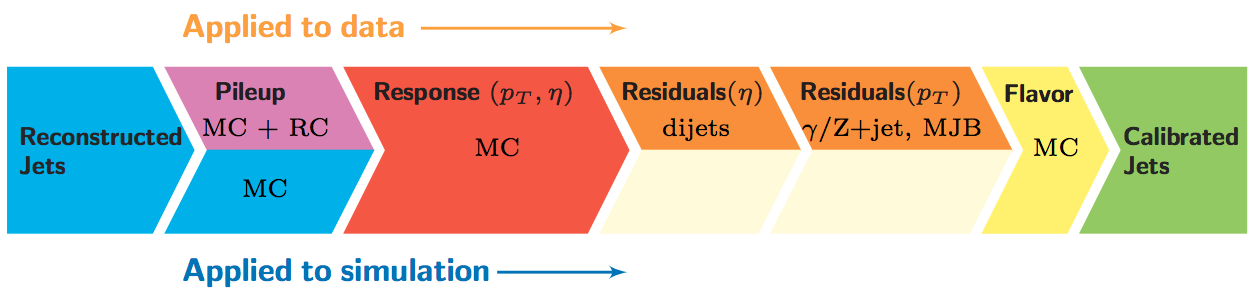
\includegraphics[width=0.8\textwidth]{/Users/db0268/Desktop/Thesis/Figures/Event_JESFlow.png}
	\caption[A schematic showing the factorised steps to correct the energy scale of a jet. These consist of a pileup correction, detector response correction with additional residuals applied in data and optional flavour corrections.]{A schematic showing the factorised steps to correct the energy scale of a jet. These consist of a pileup correction, detector response correction with additional residuals applied in data and optional flavour corrections. Schematic taken from~\cite{Event:JEC}.}
	\label{fig:JESFlow}
\end{figure}

The first correction is applied to counter additional energy in the jet, known as \textit{offset energy}, coming from pileup and the underlying event. 
%+noise
In-time pileup is already partially removed by the charged hadron subtraction algorithm, which accounts for $\sim50\%$ of the offset energy.
The rest of the diffuse neutral energy and out-of-time pileup is removed on an event-by-event basis using the \textit{hybrid jet area method} dependent on the offset energy density $\rho$ and the effective jet area $A^{\mathrm{jet}}$.
The variable $\rho$ is taken as the median of the energies present in a grid of $\eta - \phi$ cells.
The use of the median creates an insensitivity to hard jets in the event.   
The correction is applied as
\begin{equation}
	\pt^{\mathrm{corr}} = \pt^{\mathrm{uncorr}} - \
	A^{\mathrm{jet}}\Big(\rho_{0}(\eta) + \
	\rho\beta(\eta)[1+\gamma(\eta)\log{(\pt^{\mathrm{uncorr}})]\Big)},
\end{equation}
where $\rho_{0}, \beta$ and $\gamma$ are $\eta$ dependent variables which are estimated from simulated \acrshort{qcd} dijets processed with and without pileup overlay and parametrise the shape of the offset energy distribution.
Residual corrections applied to data which stem from differences between the data and the detector simulation are determined using the random cone method on zero-bias events.
% data and simulation of rho???
Zero-bias events are events in which there is no hard-scattering process and so any jet energies should come from pileup provided the electronic noise is small.
The random cone method estimates $\rho$ by clustering many jets around random cones mapping all $\eta-\phi$ space and taking the average jet \pt{}.
This correction removes any dependence of the jet energy on the luminosity for the subsequent corrections.
% ue contained in rho0, 
% correction for nonuniformity in IT and OOT offsets wrt eta, beta
% residual correction factor depending on log jet pt dependence, gamma

Next, a second set of corrections are applied to both data and simulation to create a uniform jet energy response with respect to \pt{} and $\eta$.
This is done using a simulated \acrshort{qcd} dijet sample to compare the \pt{} of the reconstructed jets to the particle-level jets.
The response is defined as the ratio of the average reconstructed jet \pt{} to the average particle-level jet \pt{}.
The simulated jet response at the end of Run I, which is used in the \acrshort{jec} applied in this thesis, can be seen in Fig.~\ref{fig:JES}.
Preliminary measurements of the simulated jet energy response for detector conditions during 2016 are given in~\cite{Event:JEC2016RunII}.
\begin{figure}[htpb!]
	\centering
	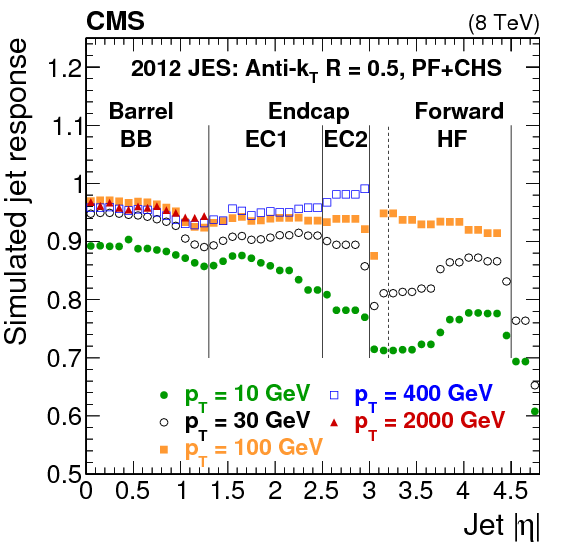
\includegraphics[width=0.55\textwidth]{/Users/db0268/Desktop/Thesis/Figures/Event_JESused.png}
	\caption[The simulated jet energy response as a function of \pt{} and $\eta$. These corrections are based on the status of the detector after the end of Run I.]{The simulated jet energy response as a function of \pt{} and $\eta$. These corrections are based on the status of the detector after the end of Run I~\cite{Event:JEC}.}
	\label{fig:JES}
\end{figure}

Residual corrections are calculated from data and applied to correct small differences seen in the jet energy response between simulation and data.
These consist of a $\eta$ dependent correction determined from \acrshort{qcd} dijet events relative to a barrel reference jet of similar \pt{} and a correction on jet energy scale with respect to \pt{}.
The \pt{} correction is based on \Zboson/\photon{}+jets and \acrshort{qcd} multijet events. 
Finally, optional corrections based on the response of different particle flavours can be applied.
These corrections are derived from simulation and are not applied in this thesis.

As well as variations present in the jet energy scale, variations are also present in the jet energy resolution (\acrshort{jer}).
The \acrshort{jer} scale factors $\mathrm{SF}_{\mathrm{JER}}$ are determined from the ratio of data to simulated \acrshort{qcd} dijet events with respect to \pt{}, $\eta$ and additional interaction vertices.
The \acrshort{jer} of jets in simulation $\sigma_\mathrm{JER}^{\mathrm{sim}}$ is also better than that seen in data and so must be smeared to match.
A hybrid of two approaches is used to correct and smear the resolution in simulation.
If a reconstructed jet is well matched to a particle-level jet such that 
\begin{equation*}
	\Delta R < \frac{R_\mathrm{cone}}{2}
\end{equation*}
and 
\begin{equation}
	\abs{\pt - \pt^\mathrm{ptcl}} < 3\,\sigma_\mathrm{JER}^{\mathrm{sim}}\,\pt,
\end{equation}
 then the jet \pt{} is rescaled by
\begin{equation*}
	1+(\mathrm{SF}_{\mathrm{JER}}-1)\frac{\pt-\pt^{\mathrm{ptcl}}}{\pt}.
\end{equation*}
However, if the jet is not matched then a stochastic smearing is applied
\begin{equation*}
	1 + \mathcal N(0,\sigma_\mathrm{JER}^{\mathrm{sim}}) \sqrt{\max(\mathrm{SF}_{\mathrm{JER}}^2 - 1, 0)}.
\end{equation*}
$\mathcal N(0,\sigma_\mathrm{JER}^{\mathrm{sim}})$ represents a random number sampled from a Gaussian distribution centred on 0 with a standard deviation given by the \acrshort{jer} in simulation.

% be careful  - this is the relative JER so Delta pt over pt
% section jet_energy_corrections (end)
% \begin{figure}[htpb]
% 	\centering
% 	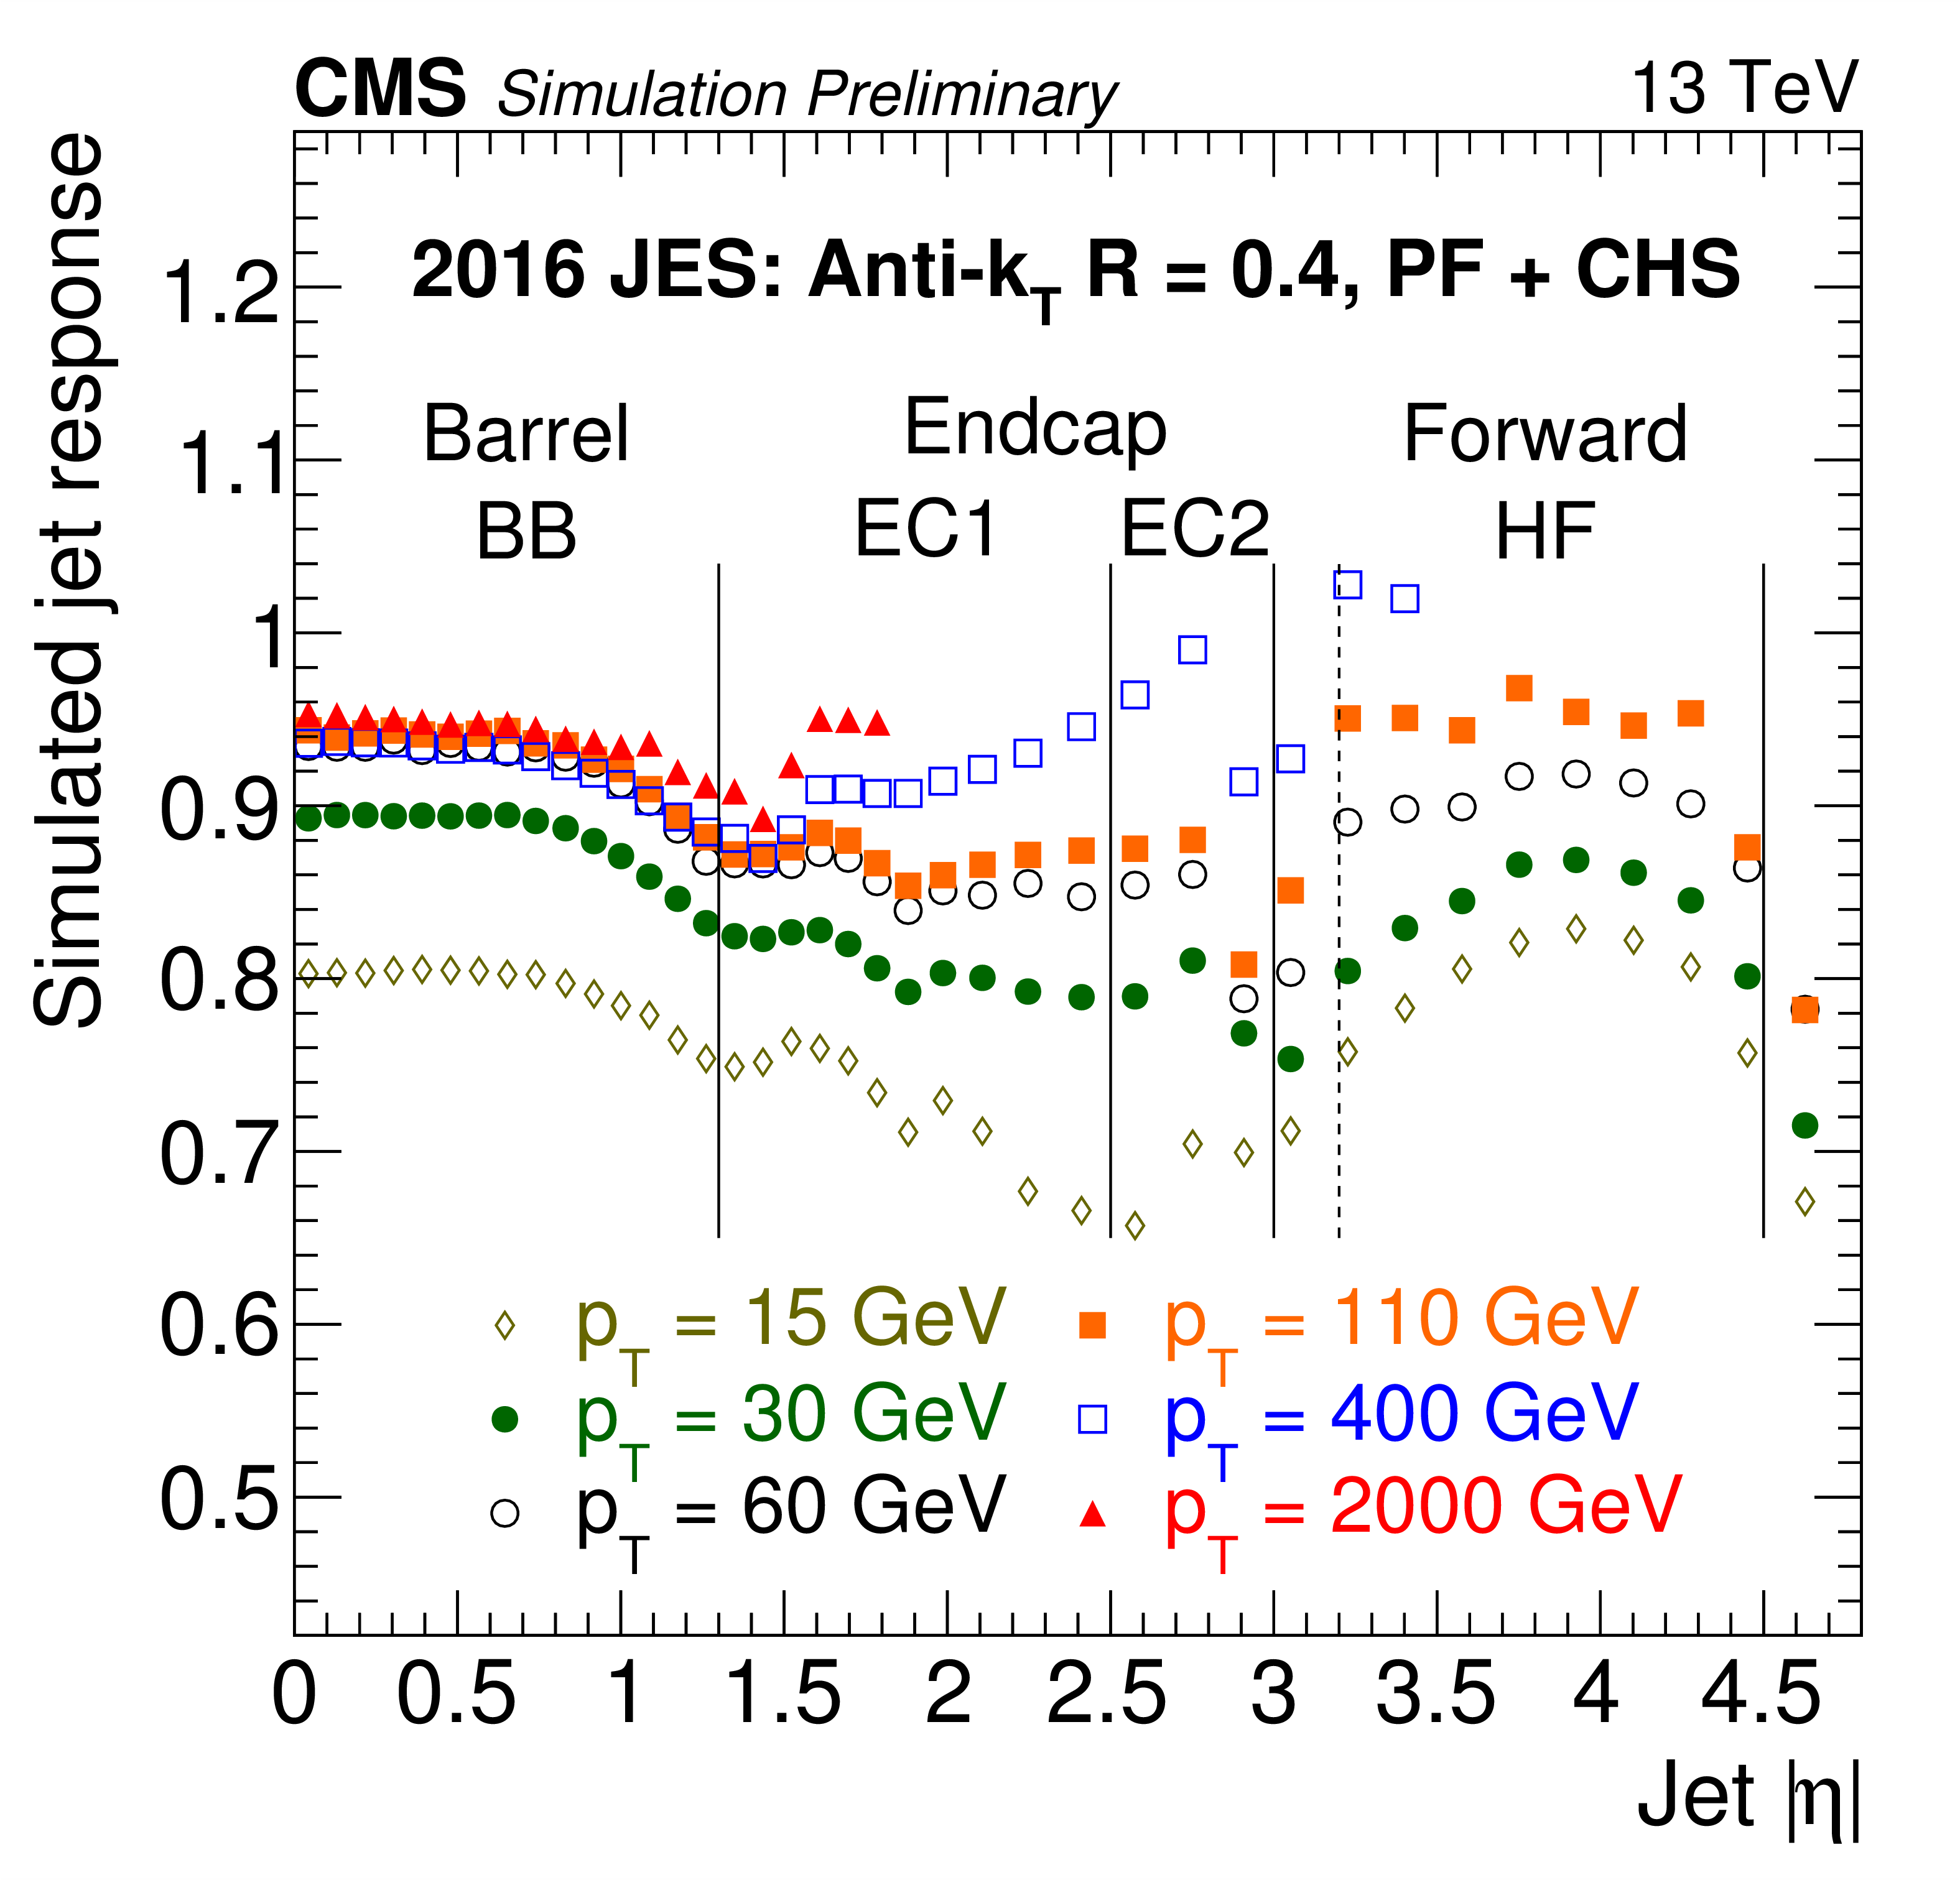
\includegraphics[width=0.49\textwidth]{/Users/db0268/Desktop/Thesis/Figures/Event_JES.png}
% 	\caption[.]{.~\cite{JEC2016RunII}}
% 	\label{fig:JES2016RunII}
% \end{figure}

\section{Reweighting from additional interactions} % (fold)
\label{sub:reweighting_from_additional_interactions}

The number of additional interactions in simulation differs to that seen in data.
The left panel of Fig.~\ref{fig:PU} shows the difference seen in the number of reconstructed vertices after full event selection.
The true vertex multiplicity distribution in simulation is reweighted to match that seen in data.
This is done by creating a scale factor from the number of additional interactions seen in data and simulation.
The true distribution of the number of additional interactions in data $N_{\mathrm{PU}}^{\mathrm{Data}}$ is estimated every bunch crossing using
\begin{equation*}
	N_{i}^{\mathrm{True}} = \sigma_{\mathrm{minbias}} \times \Lum_{i}.
\end{equation*}
The parameter $\sigma_{\mathrm{minbias}}$ is the total inelastic cross section taken as 69.2\mb{} and $\Lum_{i}$ the instantaneous luminosity in the luminosity section $i$.
The true distribution of additional interactions in simulation $N_{\mathrm{PU}}^{\mathrm{Sim}}$ also includes interactions from out-of-time pileup.
The number of reconstructed vertices in simulation is then reweighted by 
\begin{equation}
	\frac{N_{\mathrm{PU}}^{\mathrm{Data}}}{N_{\mathrm{PU}}^{\mathrm{Sim}}},
\end{equation}
and the application is shown in the right panel of Fig.~\ref{fig:PU}.
While a discrepancy is seen in the reweighting, the distributions of the vertex multiplicities matches when considering the uncertainties on $\sigma_{\mathrm{minbias}}$ ($\pm4.6\%$).

\begin{figure}[htpb]
	\centering
	\includegraphics[width=0.49\textwidth]{/Users/db0268/Mount/SoolinScratch/DPS/DPSTestingGround/DailyPythonScripts/data_thesis/plots/control_plots/Nominal/Control/Ref_selection/COMBINED_NPUNoWeight_2orMoreBtags_with_ratio}
	\includegraphics[width=0.49\textwidth]{/Users/db0268/Mount/SoolinScratch/DPS/DPSTestingGround/DailyPythonScripts/data_thesis/plots/control_plots/Nominal/Control/Ref_selection/COMBINED_NPU_2orMoreBtags_with_ratio}
	\caption[A plot showing the distribution of the number of reconstructed primary vertices in simulation and data. The left panel shows the distribution before pileup reweighting and the right panel after.]{A plot showing the distribution of the number of reconstructed primary vertices in simulation and data. The left panel shows the distribution before pileup reweighting and the right panel after.}
	\label{fig:PU}
\end{figure}
% again minbias = total inelastic cross section, L = instantaneous Lumi.
% Alternate method is to count number of reconstructed primary vertices in a series of events. The average number of additional vertices corresponds linearly to the number of additional interactions, modulo the ~70% vertex reconstruction efficiency. So, the average number of reconstructed vertices divided by 0.7 is a good estimate of the number of additional interactions present in one LumiSection.
% section reweighting_from_additional_interactions (end)

\section{Reweighting from b jet identification} % (fold)
\label{sub:reweighting_from_b_jet_identification}

% The CSVv2 algorithm response of jets in data and simulation is not equivalent and so scale factors, derived in TODO, are applied 
% WP-> 70pc eff. Calc our own->70pc
The \bquark{} jet identification efficiencies for a given configuration of jets in data and simulation are different.
The simulation is corrected to match data by applying a weight
\begin{equation*}
	w = \frac{P(\mathrm{Data})}{P(\mathrm{Sim})},
\end{equation*}
where
\begin{equation*}
	P(\mathrm{Sim}) = \prod_{i\text{ = tagged}}\epsilon_{i}\prod_{j\text{ = not tagged}}(1 - \epsilon_{j})
\end{equation*}
and
\begin{equation*}
	P(\mathrm{Data}) = \prod_{i\text{ = tagged}}\mathrm{SF}_{i}\epsilon_{i}\prod_{j\text{ = not tagged}}(1 - \mathrm{SF}_{j}\epsilon_{j}).
\end{equation*}
The parameters $\epsilon_{i}$ and $\mathrm{SF}_{i}$ are the \bquark{} quark tagging efficiency and scale factor ($\epsilon_{\mathrm{DATA}}/\epsilon_{\mathrm{MC}}$) for the jet $i$, respectively.
The scale factors applied to the \bquark{} and light flavour jets in this thesis are derived in~\cite{Event:BTV}.

Both the \bquark{} tagging scale factors and efficiencies are calculated and applied as functions of \pt{}, $\eta$ and flavour (\bquark{}, \cquark{}, \udsg{}).
The \bquark{} jet tagging efficiency and light jet mis-tagging efficiencies are calculated from the \powhegpythia{} \ttbar{} simulation.
They are taken as the fraction of tagged jets over the total number of \bquark{} jets.
Figure~\ref{fig:BTag} shows the \bquark{} quark jet tagging efficiencies, which for genuine \bquark{} jets is $\approx70\%$ and for misidentified jets from light quarks is $\approx1\%$.
\begin{figure}[htpb]
	\centering
	\includegraphics[width=0.49\textwidth]{/Users/db0268/Mount/SoolinScratch/DPS/DPSTestingGround/DailyPythonScripts/plots/BTagEfficiency/pt_efficiency}
	\includegraphics[width=0.49\textwidth]{/Users/db0268/Mount/SoolinScratch/DPS/DPSTestingGround/DailyPythonScripts/plots/BTagEfficiency/eta_efficiency}
	\caption[The left panel shows the \bquark{} tagging efficiency with respect to jet \pt{} and the right panel with respect to jet $\eta$. Both panels show the efficiencies separated into \bquark{}, \cquark{} and light flavours.]{The left panel shows the \bquark{} tagging efficiency with respect to jet \pt{} and the right panel with respect to jet $\eta$. Both panels show the efficiencies separated into \bquark{}, \cquark{} and light flavours.}
	\label{fig:BTag}
\end{figure}

Figure~\ref{fig:BWeight} shows the \bquark{} jet multiplicity after full event selection before applying the \bquark{} jet reweighting in the left panel and after in the right panel.
The discrepancy in the first bin is covered by the uncertainty in multijet \acrshort{qcd}, taken from simulation.
The size of the multijet \acrshort{qcd} normalisation uncertainty is $\approx60\%$ motivated in Sec.~\ref{sec:multijet_qcd}.
\begin{figure}[htpb]
	\centering
	\includegraphics[width=0.49\textwidth]{/Users/db0268/Mount/SoolinScratch/DPS/DPSTestingGround/DailyPythonScripts/data_thesis/plots/control_plots/Nominal/Control/Ref_selection/COMBINED_NBJetsNoWeight_2orMoreBtags_with_ratio}
	\includegraphics[width=0.49\textwidth]{/Users/db0268/Mount/SoolinScratch/DPS/DPSTestingGround/DailyPythonScripts/data_thesis/plots/control_plots/Nominal/Control/Ref_selection/COMBINED_NBJets_2orMoreBtags_with_ratio}	
	\caption[The left panel shows the \bquark{} jet multiplicity distribution before reweighting and the right panel after reweighting.]{The left panel shows the \bquark{} jet multiplicity distribution before reweighting and the right panel after reweighting.}
	\label{fig:BWeight}
\end{figure}
% section reweighting_from_b_jet_identification (end)

\section{Reweighting from leptons} % (fold)
\label{sub:reweighting_from_leptons}

The reconstruction, identification and triggering efficiencies of leptons are measured in data and corrected in simulation to match data.
The electron efficiencies and scale factors are derived using the tag-and-probe method following prescriptions defined in~\cite{Event:eSFMethod} using the clustering algorithm described in~\cite{Event:PFlow} and are presented in~\cite{Event:ElectronSF}.
Muon scale factors are measured in a similar manner and are presented in~\cite{Event:MuonSF,Event:MuonTrigSF}.
In both channels the efficiencies are measured from events containing a \Zboson{} boson and the corrective scale factors are applied as a function of \pt{} and supercluster pseudorapidity \sceta{}.
The total lepton scale factors vary between 0.95 and 1.

The electron \acrshort{id} scale factors are produced in bins of \sceta{} coarse enough to have significant effects on the distribution of \LETA{}.
This is because the high resolution of \LETA{} allows for fine-bin measurements and the application of the scale factors would cover several bins.
It is therefore not appropriate to use these electron \acrshort{id} scale factors for the \LETA{} event variable.
They are rederived with respect to the finer binning used in the production of the electron reconstruction scale factors for an identical \pt{} range.
An identical method used for the original scale factors is used in the rederivation.
Figure~\ref{fig:eIDSF} shows the efficiency of the electron \acrshort{id} in data (points) and simulation (dashes) and the scale factor to be applied is the ratio.
This new scale factor is only applied for the \LETA{} differential measurements.
\begin{figure}[htpb]
	\centering
	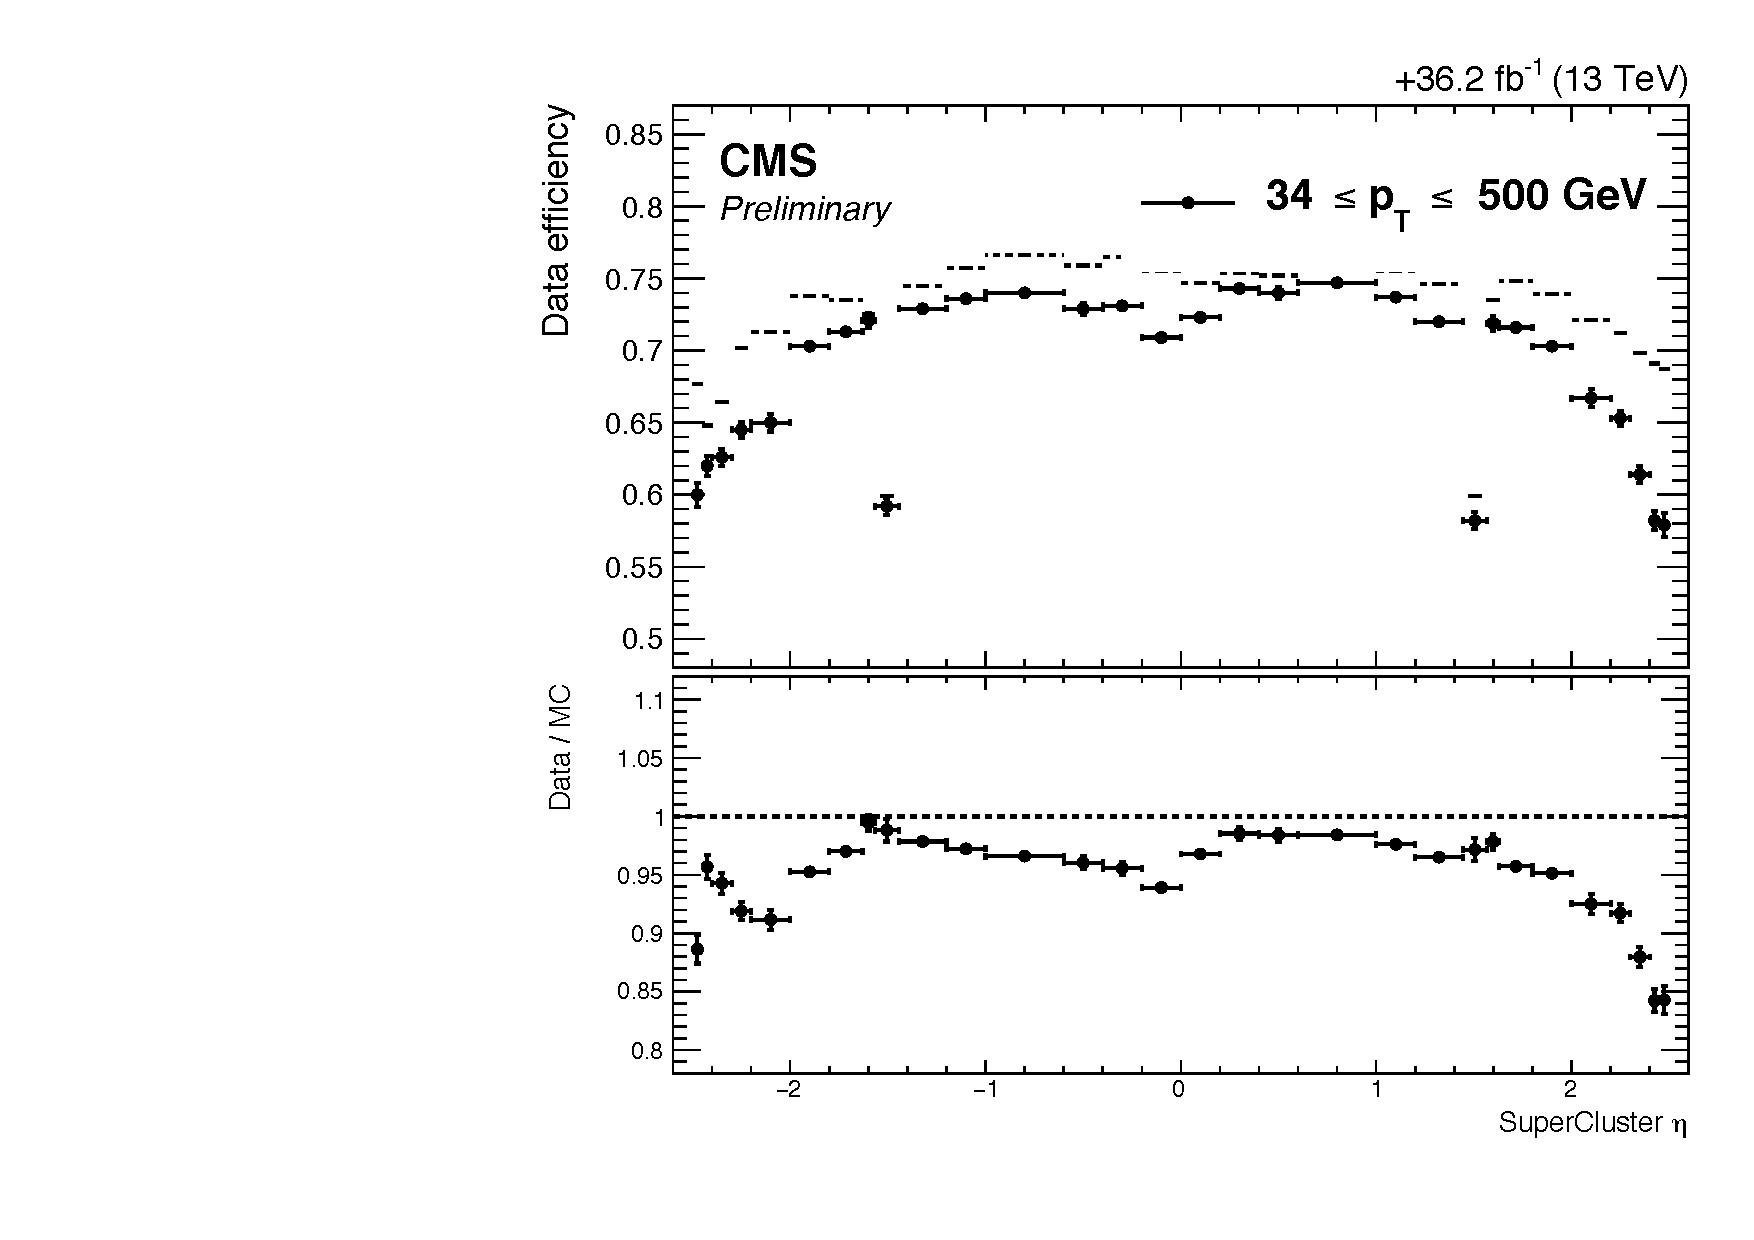
\includegraphics[width=0.7\textwidth]{Figures/Event_eIDSF.pdf}
	\caption[The electron identification efficiency for data and simulation calculated with events with a \Zboson{} boson present using the tag-and-probe method. The ratio of the two efficiencies is the finer binned scale factors applied in the \LETA{} measurements.]{The electron identification efficiency for data and simulation calculated with events with a \Zboson{} boson present using the tag-and-probe method. The ratio of the two efficiencies is the finer binned scale factors applied in the \LETA{} measurements.}
	\label{fig:eIDSF}
\end{figure}
% section reweighting_from_leptons (end)

\section{Multijet \acrshort{qcd}} % (fold)
\label{sec:multijet_qcd}

The multijet \acrshort{qcd} background is notoriously hard to model and as such a data driven approach is used to estimate its contribution in the signal region from an orthogonal control region.
The control region is designed to be enhanced in multijet \acrshort{qcd} and to achieve that in the \eJets{} channel the \acrshort{qcd} event selection inverts the isolation requirement in the electron \acrshort{id} and requires exactly zero \bquark{} jets.
For the \muJets{} channel the control region event selection requires $0.15<\Irel<0.30$ and zero \bquark{} tagged jets.
In these control regions, the contribution of \ttbar{}, single top quark, and \Vjets{} background is estimated from simulation to be $\approx15-20\%$.
These estimations are subtracted from the data to extract the shape of the multijet \acrshort{qcd} in data.
The \acrshort{qcd} distributions are then scaled to the signal region by a transfer factor derived from simulation
\begin{equation*}
	t_{f}=\frac{N^{\mathrm{Signal}}_{\QCD,\,\mathrm{MC}}}{N^{\mathrm{Control}}_{\QCD,\,\mathrm{MC}}},
\end{equation*}
where $N^{\mathrm{Signal}}_{\QCD,\,\mathrm{MC}}$ and $N^{\mathrm{Control}}_{\QCD,\,\mathrm{MC}}$ are the total normalisation of the \acrshort{qcd} simulation in the signal and control regions respectively.
Transfer factors for all nominal control regions are shown in Tab.~\ref{tb:qcdTF}.
\begin{table}[h!]
    \centering
    \caption{The transfer factors to the signal region from the four multijet \QCD{} control regions.}
    \label{tb:qcdTF}
    \begin{tabular}{lc}
            \textbf{Control region}     			&	\textbf{Transfer factor} \\
            \hline
            Non-isolated electron					&	0.27 \\
            Conversion electron						&   0.03 \\
            Non-isolated muon $0.15<\Irel<0.30 $ 	& 	0.11 \\
            Non-isolated muon $0.30<\Irel<\infty$ 	& 	0.08 \\
    \end{tabular} \\
\end{table}


To validate the use of the nominal control region, the \acrshort{qcd} contribution is estimated in an alternate control region and compared to background subtracted data in that control region.
The comparison can also yield the shape and normalisation uncertainties on the data driven \acrshort{qcd} estimate.
In the \eJets{} channel the alternate control region uses an electron ID where the conversion veto or missing hits criteria has been inverted and in the \muJets{} channel the $0.30<\Irel<\infty$ region is used.
Both still require exactly zero \bquark{} tagged jets.
The data-simulation comparison plots of the event variables in the multijet \acrshort{qcd} control regions for the \eJets{} channel are shown in Figs.~\ref{fig:QCDeNonIso} and~\ref{fig:QCDeConv} and for the \muJets{} channel in Figs.~\ref{fig:QCDmuNonIso2} and~\ref{fig:QCDmuNonIso}.

Figures~\ref{fig:QCDeValid} and~\ref{fig:QCDmuValid} show the data-driven \acrshort{qcd} estimates in the alternate control region compared to the \acrshort{qcd} calculated by subtracting backgrounds from the data in the alternate control region.
The differences between the two predictions show the accuracy of the prediction, which is expected to be similar for the prediction in the signal region.
The uncertainty of the \acrshort{qcd} prediction in the signal region can therefore be taken from the discrepancies seen in this control region.
Any offset from unity in the ratio of the two \acrshort{qcd} yields gives the normalisation uncertainty, taken as $\pm60\%$ (gold band) and the spread of the ratio gives the shape uncertainty, taken as $\pm30\%$ (grey band).
The regions where the ratio is outside these uncertainty bands the expected contribution of \acrshort{qcd} is negligible, \eg{} at high \ptmiss{}.
\begin{figure}[hp!]
	\centering
	\includegraphics[width=0.32\textwidth]{/Users/db0268/Mount/SoolinScratch/DPS/DPSTestingGround/DailyPythonScripts/data_thesis/plots/control_plots/Nominal/QCDControl/electronQCDNonIso/electronQCDNonIso_logYNJets_0btag_with_ratio.png}
	\includegraphics[width=0.32\textwidth]{/Users/db0268/Mount/SoolinScratch/DPS/DPSTestingGround/DailyPythonScripts/data_thesis/plots/control_plots/Nominal/QCDControl/electronQCDNonIso/electronQCDNonIso_HT_0btag_with_ratio.png}
	\includegraphics[width=0.32\textwidth]{/Users/db0268/Mount/SoolinScratch/DPS/DPSTestingGround/DailyPythonScripts/data_thesis/plots/control_plots/Nominal/QCDControl/electronQCDNonIso/electronQCDNonIso_ST_0btag_with_ratio.png} \\
	\includegraphics[width=0.32\textwidth]{/Users/db0268/Mount/SoolinScratch/DPS/DPSTestingGround/DailyPythonScripts/data_thesis/plots/control_plots/Nominal/QCDControl/electronQCDNonIso/electronQCDNonIso_MET_0btag_with_ratio.png}
	\includegraphics[width=0.32\textwidth]{/Users/db0268/Mount/SoolinScratch/DPS/DPSTestingGround/DailyPythonScripts/data_thesis/plots/control_plots/Nominal/QCDControl/electronQCDNonIso/electronQCDNonIso_WPT_0btag_with_ratio.png} \\
	\includegraphics[width=0.32\textwidth]{/Users/db0268/Mount/SoolinScratch/DPS/DPSTestingGround/DailyPythonScripts/data_thesis/plots/control_plots/Nominal/QCDControl/electronQCDNonIso/electronQCDNonIso_LeptonPt_0btag_with_ratio.png} 
	\includegraphics[width=0.32\textwidth]{/Users/db0268/Mount/SoolinScratch/DPS/DPSTestingGround/DailyPythonScripts/data_thesis/plots/control_plots/Nominal/QCDControl/electronQCDNonIso/electronQCDNonIso_AbsLeptonEta_0btag_with_ratio.png}
	\includegraphics[width=0.32\textwidth]{/Users/db0268/Mount/SoolinScratch/DPS/DPSTestingGround/DailyPythonScripts/data_thesis/plots/control_plots/Nominal/QCDControl/electronQCDNonIso/electronQCDNonIso_relIso_0btag_with_ratio.png}
	\caption[The distributions of the event variables and $I_{\mathrm{rel}}$ in the non-isolated electron control region. The ratio of the number of events in data to that in simulation is shown below each of the distributions, with the statistical uncertainty in data given by the vertical error bars.]{The distributions of the event variables and $I_{\mathrm{rel}}$ in the non-isolated electron control region. The ratio of the number of events in data to that in simulation is shown below each of the distributions, with the statistical uncertainty in data given by the vertical error bars.}
	\label{fig:QCDeNonIso}
\end{figure}
\begin{figure}[hp!]
	\centering
	\includegraphics[width=0.32\textwidth]{/Users/db0268/Mount/SoolinScratch/DPS/DPSTestingGround/DailyPythonScripts/data_thesis/plots/control_plots/Nominal/QCDControl/electronQCDConversions/electronQCDConversions_logYNJets_0btag_with_ratio.png}
	\includegraphics[width=0.32\textwidth]{/Users/db0268/Mount/SoolinScratch/DPS/DPSTestingGround/DailyPythonScripts/data_thesis/plots/control_plots/Nominal/QCDControl/electronQCDConversions/electronQCDConversions_HT_0btag_with_ratio.png}
	\includegraphics[width=0.32\textwidth]{/Users/db0268/Mount/SoolinScratch/DPS/DPSTestingGround/DailyPythonScripts/data_thesis/plots/control_plots/Nominal/QCDControl/electronQCDConversions/electronQCDConversions_ST_0btag_with_ratio.png} \\
	\includegraphics[width=0.32\textwidth]{/Users/db0268/Mount/SoolinScratch/DPS/DPSTestingGround/DailyPythonScripts/data_thesis/plots/control_plots/Nominal/QCDControl/electronQCDConversions/electronQCDConversions_MET_0btag_with_ratio.png}
	\includegraphics[width=0.32\textwidth]{/Users/db0268/Mount/SoolinScratch/DPS/DPSTestingGround/DailyPythonScripts/data_thesis/plots/control_plots/Nominal/QCDControl/electronQCDConversions/electronQCDConversions_WPT_0btag_with_ratio.png} \\
	\includegraphics[width=0.32\textwidth]{/Users/db0268/Mount/SoolinScratch/DPS/DPSTestingGround/DailyPythonScripts/data_thesis/plots/control_plots/Nominal/QCDControl/electronQCDConversions/electronQCDConversions_LeptonPt_0btag_with_ratio.png} 
	\includegraphics[width=0.32\textwidth]{/Users/db0268/Mount/SoolinScratch/DPS/DPSTestingGround/DailyPythonScripts/data_thesis/plots/control_plots/Nominal/QCDControl/electronQCDConversions/electronQCDConversions_AbsLeptonEta_0btag_with_ratio.png}
	\includegraphics[width=0.32\textwidth]{/Users/db0268/Mount/SoolinScratch/DPS/DPSTestingGround/DailyPythonScripts/data_thesis/plots/control_plots/Nominal/QCDControl/electronQCDConversions/electronQCDConversions_relIso_0btag_with_ratio.png}
	\caption[The distributions of the event variables and $I_{\mathrm{rel}}$ in the conversion electron control region. The ratio of the number of events in data to that in simulation is shown below each of the distributions, with the statistical uncertainty in data given by the vertical error bars.]{The distributions of the event variables and $I_{\mathrm{rel}}$ in the conversion electron control region. The ratio of the number of events in data to that in simulation is shown below each of the distributions, with the statistical uncertainty in data given by the vertical error bars.}
	\label{fig:QCDeConv}
\end{figure}
\begin{figure}[hp!]
	\centering
	\includegraphics[width=0.32\textwidth]{/Users/db0268/Mount/SoolinScratch/DPS/DPSTestingGround/DailyPythonScripts/data_thesis/plots/control_plots/Nominal/QCDControl/muonQCDNonIso2/muonQCDNonIso2_logYNJets_0btag_with_ratio.png}
	\includegraphics[width=0.32\textwidth]{/Users/db0268/Mount/SoolinScratch/DPS/DPSTestingGround/DailyPythonScripts/data_thesis/plots/control_plots/Nominal/QCDControl/muonQCDNonIso2/muonQCDNonIso2_HT_0btag_with_ratio.png}
	\includegraphics[width=0.32\textwidth]{/Users/db0268/Mount/SoolinScratch/DPS/DPSTestingGround/DailyPythonScripts/data_thesis/plots/control_plots/Nominal/QCDControl/muonQCDNonIso2/muonQCDNonIso2_ST_0btag_with_ratio.png} \\
	\includegraphics[width=0.32\textwidth]{/Users/db0268/Mount/SoolinScratch/DPS/DPSTestingGround/DailyPythonScripts/data_thesis/plots/control_plots/Nominal/QCDControl/muonQCDNonIso2/muonQCDNonIso2_MET_0btag_with_ratio.png}
	\includegraphics[width=0.32\textwidth]{/Users/db0268/Mount/SoolinScratch/DPS/DPSTestingGround/DailyPythonScripts/data_thesis/plots/control_plots/Nominal/QCDControl/muonQCDNonIso2/muonQCDNonIso2_WPT_0btag_with_ratio.png} \\
	\includegraphics[width=0.32\textwidth]{/Users/db0268/Mount/SoolinScratch/DPS/DPSTestingGround/DailyPythonScripts/data_thesis/plots/control_plots/Nominal/QCDControl/muonQCDNonIso2/muonQCDNonIso2_LeptonPt_0btag_with_ratio.png} 
	\includegraphics[width=0.32\textwidth]{/Users/db0268/Mount/SoolinScratch/DPS/DPSTestingGround/DailyPythonScripts/data_thesis/plots/control_plots/Nominal/QCDControl/muonQCDNonIso2/muonQCDNonIso2_AbsLeptonEta_0btag_with_ratio.png}
	\includegraphics[width=0.32\textwidth]{/Users/db0268/Mount/SoolinScratch/DPS/DPSTestingGround/DailyPythonScripts/data_thesis/plots/control_plots/Nominal/QCDControl/muonQCDNonIso2/muonQCDNonIso2_relIso_0btag_with_ratio.png}
	\caption[The distributions of the event variables and $I_{\mathrm{rel}}$ in the non-isolated $(0.15 < I_{\mathrm{rel}} < 0.30)$ muon control region. The ratio of the number of events in data to that in simulation is shown below each of the distributions, with the statistical uncertainty in data given by the vertical error bars.]{The distributions of the event variables and $I_{\mathrm{rel}}$ in the non-isolated $(0.15 < I_{\mathrm{rel}} < 0.30)$ muon control region. The ratio of the number of events in data to that in simulation is shown below each of the distributions, with the statistical uncertainty in data given by the vertical error bars.}
	\label{fig:QCDmuNonIso2}
\end{figure}
\begin{figure}[hp!]
	\centering
	\includegraphics[width=0.32\textwidth]{/Users/db0268/Mount/SoolinScratch/DPS/DPSTestingGround/DailyPythonScripts/data_thesis/plots/control_plots/Nominal/QCDControl/muonQCDNonIso/muonQCDNonIso_logYNJets_0btag_with_ratio.png}
	\includegraphics[width=0.32\textwidth]{/Users/db0268/Mount/SoolinScratch/DPS/DPSTestingGround/DailyPythonScripts/data_thesis/plots/control_plots/Nominal/QCDControl/muonQCDNonIso/muonQCDNonIso_HT_0btag_with_ratio.png}
	\includegraphics[width=0.32\textwidth]{/Users/db0268/Mount/SoolinScratch/DPS/DPSTestingGround/DailyPythonScripts/data_thesis/plots/control_plots/Nominal/QCDControl/muonQCDNonIso/muonQCDNonIso_ST_0btag_with_ratio.png} \\
	\includegraphics[width=0.32\textwidth]{/Users/db0268/Mount/SoolinScratch/DPS/DPSTestingGround/DailyPythonScripts/data_thesis/plots/control_plots/Nominal/QCDControl/muonQCDNonIso/muonQCDNonIso_MET_0btag_with_ratio.png}
	\includegraphics[width=0.32\textwidth]{/Users/db0268/Mount/SoolinScratch/DPS/DPSTestingGround/DailyPythonScripts/data_thesis/plots/control_plots/Nominal/QCDControl/muonQCDNonIso/muonQCDNonIso_WPT_0btag_with_ratio.png} \\
	\includegraphics[width=0.32\textwidth]{/Users/db0268/Mount/SoolinScratch/DPS/DPSTestingGround/DailyPythonScripts/data_thesis/plots/control_plots/Nominal/QCDControl/muonQCDNonIso/muonQCDNonIso_LeptonPt_0btag_with_ratio.png} 
	\includegraphics[width=0.32\textwidth]{/Users/db0268/Mount/SoolinScratch/DPS/DPSTestingGround/DailyPythonScripts/data_thesis/plots/control_plots/Nominal/QCDControl/muonQCDNonIso/muonQCDNonIso_AbsLeptonEta_0btag_with_ratio.png}
	\includegraphics[width=0.32\textwidth]{/Users/db0268/Mount/SoolinScratch/DPS/DPSTestingGround/DailyPythonScripts/data_thesis/plots/control_plots/Nominal/QCDControl/muonQCDNonIso/muonQCDNonIso_relIso_0btag_with_ratio.png}
	\caption[The distributions of the event variables and $I_{\mathrm{rel}}$ in the non-isolated $(0.30 < I_{\mathrm{rel}} < \infty )$ muon control region. The ratio of the number of events in data to that in simulation is shown below each of the distributions, with the statistical uncertainty in data given by the vertical error bars.]{The distributions of the event variables and $I_{\mathrm{rel}}$ in the non-isolated $(0.30 < I_{\mathrm{rel}} < \infty )$ muon control region. The ratio of the number of events in data to that in simulation is shown below each of the distributions, with the statistical uncertainty in data given by the vertical error bars.}
	\label{fig:QCDmuNonIso}
\end{figure}

\begin{figure}[p]
	\centering
	\includegraphics[width=0.32\textwidth]{/Users/db0268/Mount/SoolinScratch/DPS/DPSTestingGround/DailyPythonScripts/plots/QCDvalidation/NJets_electron.pdf}
	\includegraphics[width=0.32\textwidth]{/Users/db0268/Mount/SoolinScratch/DPS/DPSTestingGround/DailyPythonScripts/plots/QCDvalidation/HT_electron.pdf} 
	\includegraphics[width=0.32\textwidth]{/Users/db0268/Mount/SoolinScratch/DPS/DPSTestingGround/DailyPythonScripts/plots/QCDvalidation/ST_electron.pdf} \\
	\includegraphics[width=0.32\textwidth]{/Users/db0268/Mount/SoolinScratch/DPS/DPSTestingGround/DailyPythonScripts/plots/QCDvalidation/MET_electron.pdf} 
	\includegraphics[width=0.32\textwidth]{/Users/db0268/Mount/SoolinScratch/DPS/DPSTestingGround/DailyPythonScripts/plots/QCDvalidation/WPT_electron.pdf} \\
	\includegraphics[width=0.32\textwidth]{/Users/db0268/Mount/SoolinScratch/DPS/DPSTestingGround/DailyPythonScripts/plots/QCDvalidation/lepton_pt_electron.pdf} 
	\includegraphics[width=0.32\textwidth]{/Users/db0268/Mount/SoolinScratch/DPS/DPSTestingGround/DailyPythonScripts/plots/QCDvalidation/abs_lepton_eta_coarse_electron.pdf}
	\caption[The prediction of multijet \QCD{} in the alternate control region from the nominal control region for each event variable in the electron channel. Also shown as a comparison is the data-subtracted \QCD{} estimate from the alternate control region. Below each of the distributions, the ratio of the two \QCD predictions is shown. This ratio gives an estimation of the \QCD{} normalisation uncertainty by the displacement from unity and was taken to be $\pm50\%$ shown by the gold band. The \QCD{} shape uncertainty is given by the spread of the ratio, taken to be $\pm30\%$ shown by the grey band.]{The prediction of multijet \QCD{} in the alternate control region from the nominal control region for each event variable in the electron channel. Also shown as a comparison is the data-subtracted \QCD{} estimate from the alternate control region. Below each of the distributions, the ratio of the two \QCD predictions is shown. This ratio gives an estimation of the \QCD{} normalisation uncertainty by the displacement from unity and was taken to be $\pm50\%$ shown by the gold band. The \QCD{} shape uncertainty is given by the spread of the ratio, taken to be $\pm30\%$ shown by the grey band.}
	\label{fig:QCDeValid}
\end{figure}

\begin{figure}[p]
	\centering
	\includegraphics[width=0.32\textwidth]{/Users/db0268/Mount/SoolinScratch/DPS/DPSTestingGround/DailyPythonScripts/plots/QCDvalidation/NJets_muon.pdf}
	\includegraphics[width=0.32\textwidth]{/Users/db0268/Mount/SoolinScratch/DPS/DPSTestingGround/DailyPythonScripts/plots/QCDvalidation/HT_muon.pdf} 
	\includegraphics[width=0.32\textwidth]{/Users/db0268/Mount/SoolinScratch/DPS/DPSTestingGround/DailyPythonScripts/plots/QCDvalidation/ST_muon.pdf} \\
	\includegraphics[width=0.32\textwidth]{/Users/db0268/Mount/SoolinScratch/DPS/DPSTestingGround/DailyPythonScripts/plots/QCDvalidation/MET_muon.pdf} 
	\includegraphics[width=0.32\textwidth]{/Users/db0268/Mount/SoolinScratch/DPS/DPSTestingGround/DailyPythonScripts/plots/QCDvalidation/WPT_muon.pdf} \\
	\includegraphics[width=0.32\textwidth]{/Users/db0268/Mount/SoolinScratch/DPS/DPSTestingGround/DailyPythonScripts/plots/QCDvalidation/lepton_pt_muon.pdf} 
	\includegraphics[width=0.32\textwidth]{/Users/db0268/Mount/SoolinScratch/DPS/DPSTestingGround/DailyPythonScripts/plots/QCDvalidation/abs_lepton_eta_coarse_muon.pdf}
	\caption[The prediction of multijet \QCD{} in the alternate control region from the nominal control region for each event variable in the muon channel. Also shown as a comparison is the data-subtracted \QCD{} estimate from the alternate control region. Below each of the distributions, the ratio of the two \QCD predictions is shown. This ratio gives an estimation of the \QCD{} normalisation uncertainty by the displacement from unity and was taken to be $\pm50\%$ shown by the gold band. The \QCD{} shape uncertainty is given by the spread of the ratio, taken to be $\pm30\%$ shown by the grey band.]{The prediction of multijet \QCD{} in the alternate control region from the nominal control region for each event variable in the muon channel. Also shown as a comparison is the data-subtracted \QCD{} estimate from the alternate control region. Below each of the distributions, the ratio of the two \QCD predictions is shown. This ratio gives an estimation of the \QCD{} normalisation uncertainty by the displacement from unity and was taken to be $\pm50\%$ shown by the gold band. The \QCD{} shape uncertainty is given by the spread of the ratio, taken to be $\pm30\%$ shown by the grey band.}
	\label{fig:QCDmuValid}
\end{figure}

% section multijet_qcd (end)
\newpage
\section{Data-simulation agreement in the signal region} % (fold)

% Figures~\ref{fig:eControlPlot1} and~\ref{fig:eControlPlot2} show the agreement between the data and the sum of the signal and background events from simulation in the \eJets{} channel and Figs.~\ref{fig:muControlPlot1} and~\ref{fig:muControlPlot2} for the \muJets{} channel.
Figures~\ref{fig:combControlPlot1} and~\ref{fig:combControlPlot2} show the agreement between the data and the sum of the signal and background events from simulation in the combined \eJets{} and \muJets{} channels.
All corrections previously described have been applied and the multijet \acrshort{qcd} contribution estimated from data.
A total of 662 381 events are measured in data, the composition of which is predicted to be $92.1\%$ \ttbar{} production, 4.4\% single top quark production, 2.1\% \Vjets{} production and 1.4\% from multijet \acrshort{qcd}.
The total level of agreement between simulation and data ($<0.2\%$) indicates the total cross section is compatible to that stated in Sec.~\ref{sub:top_quark_production}.
The statistical uncertainty in the data is given by vertical error bars.
The hatched bands shows the statistical uncertainty in the number of simulated events and experimental uncertainties combined in quadrature.
The set of experimental uncertainties include those from the \acrshort{jec} and \ptmiss{}, the luminosity, the pileup, lepton and \bquark{} tagging scale factors and the background predictions.
These uncertainties are explained in more detail in Sec.~\ref{sub:experimental_uncertainties}.
\label{sec:data_simulation_agreement_in_the_signal_region}
% \begin{figure}[hp]
% 	\centering
% 	\includegraphics[width=0.49\textwidth]{/Users/db0268/Mount/SoolinScratch/DPS/DPSTestingGround/DailyPythonScripts/data_thesis/plots/control_plots_with_systematic/logY/electron_NJets_with_ratio_logY.png} \\
% 	\includegraphics[width=0.49\textwidth]{/Users/db0268/Mount/SoolinScratch/DPS/DPSTestingGround/DailyPythonScripts/data_thesis/plots/control_plots_with_systematic/electron_HT_with_ratio.png}
% 	\includegraphics[width=0.49\textwidth]{/Users/db0268/Mount/SoolinScratch/DPS/DPSTestingGround/DailyPythonScripts/data_thesis/plots/control_plots_with_systematic/electron_ST_with_ratio.png} \\
% 	\caption[.]{.}
% 	\label{fig:eControlPlot1}
% \end{figure}
% \begin{figure}[hp]
% 	\centering
% 	\includegraphics[width=0.49\textwidth]{/Users/db0268/Mount/SoolinScratch/DPS/DPSTestingGround/DailyPythonScripts/data_thesis/plots/control_plots_with_systematic/electron_MET_with_ratio.png}
% 	\includegraphics[width=0.49\textwidth]{/Users/db0268/Mount/SoolinScratch/DPS/DPSTestingGround/DailyPythonScripts/data_thesis/plots/control_plots_with_systematic/electron_WPT_with_ratio.png} \\
% 	\includegraphics[width=0.49\textwidth]{/Users/db0268/Mount/SoolinScratch/DPS/DPSTestingGround/DailyPythonScripts/data_thesis/plots/control_plots_with_systematic/electron_lepton_pt_with_ratio.png} 
% 	\includegraphics[width=0.49\textwidth]{/Users/db0268/Mount/SoolinScratch/DPS/DPSTestingGround/DailyPythonScripts/data_thesis/plots/control_plots_with_systematic/electron_abs_lepton_eta_coarse_with_ratio.png}
% 	\caption[.]{.}
% 	\label{fig:eControlPlot2}
% \end{figure}
% \begin{figure}[hp]
% 	\centering
% 	\includegraphics[width=0.49\textwidth]{/Users/db0268/Mount/SoolinScratch/DPS/DPSTestingGround/DailyPythonScripts/data_thesis/plots/control_plots_with_systematic/logY/muon_NJets_with_ratio_logY.png} \\
% 	\includegraphics[width=0.49\textwidth]{/Users/db0268/Mount/SoolinScratch/DPS/DPSTestingGround/DailyPythonScripts/data_thesis/plots/control_plots_with_systematic/muon_HT_with_ratio.png}
% 	\includegraphics[width=0.49\textwidth]{/Users/db0268/Mount/SoolinScratch/DPS/DPSTestingGround/DailyPythonScripts/data_thesis/plots/control_plots_with_systematic/muon_ST_with_ratio.png} \\
% 	\caption[.]{.}
% 	\label{fig:muControlPlot1}
% \end{figure}
% \begin{figure}[hp]
% 	\centering
% 	\includegraphics[width=0.49\textwidth]{/Users/db0268/Mount/SoolinScratch/DPS/DPSTestingGround/DailyPythonScripts/data_thesis/plots/control_plots_with_systematic/muon_MET_with_ratio.png}
% 	\includegraphics[width=0.49\textwidth]{/Users/db0268/Mount/SoolinScratch/DPS/DPSTestingGround/DailyPythonScripts/data_thesis/plots/control_plots_with_systematic/muon_WPT_with_ratio.png} \\
% 	\includegraphics[width=0.49\textwidth]{/Users/db0268/Mount/SoolinScratch/DPS/DPSTestingGround/DailyPythonScripts/data_thesis/plots/control_plots_with_systematic/muon_lepton_pt_with_ratio.png} 
% 	\includegraphics[width=0.49\textwidth]{/Users/db0268/Mount/SoolinScratch/DPS/DPSTestingGround/DailyPythonScripts/data_thesis/plots/control_plots_with_systematic/muon_abs_lepton_eta_coarse_with_ratio.png}
% 	\caption[.]{.}
% 	\label{fig:muControlPlot2}
% \end{figure}
\begin{figure}[hp]
	\centering
	\includegraphics[width=0.49\textwidth]{/Users/db0268/Mount/SoolinScratch/DPS/DPSTestingGround/DailyPythonScripts/data_thesis/plots/control_plots_with_systematic/logY/COMBINED_NJets_with_ratio_logY.png} \\
	\includegraphics[width=0.49\textwidth]{/Users/db0268/Mount/SoolinScratch/DPS/DPSTestingGround/DailyPythonScripts/data_thesis/plots/control_plots_with_systematic/COMBINED_HT_with_ratio.png}
	\includegraphics[width=0.49\textwidth]{/Users/db0268/Mount/SoolinScratch/DPS/DPSTestingGround/DailyPythonScripts/data_thesis/plots/control_plots_with_systematic/COMBINED_ST_with_ratio.png} \\
	\caption[The distributions of \NJET{}, \HT{} and \ST{} after full event selection. The \ttbar{} simulation is normalised to the \NNLO{} prediction. The ratio of the number of events in data to that in simulation is shown below each of the distributions, with the statistical uncertainty in the data shown by the vertical error bars. The statistical uncertainty in the number of simulated events quadratically combined with the experimental uncertainties is shown by the hatched band.]{The distributions of \NJET{}, \HT{} and \ST{} after full event selection. The \ttbar{} simulation is normalised to the \NNLO{} prediction. The ratio of the number of events in data to that in simulation is shown below each of the distributions, with the statistical uncertainty in the data shown by the vertical error bars. The statistical uncertainty in the number of simulated events quadratically combined with the experimental uncertainties is shown by the hatched band.}
	\label{fig:combControlPlot1}
\end{figure}
\begin{figure}[hp]
	\centering
	\includegraphics[width=0.49\textwidth]{/Users/db0268/Mount/SoolinScratch/DPS/DPSTestingGround/DailyPythonScripts/data_thesis/plots/control_plots_with_systematic/COMBINED_MET_with_ratio.png}
	\includegraphics[width=0.49\textwidth]{/Users/db0268/Mount/SoolinScratch/DPS/DPSTestingGround/DailyPythonScripts/data_thesis/plots/control_plots_with_systematic/COMBINED_WPT_with_ratio.png} \\
	\includegraphics[width=0.49\textwidth]{/Users/db0268/Mount/SoolinScratch/DPS/DPSTestingGround/DailyPythonScripts/data_thesis/plots/control_plots_with_systematic/COMBINED_lepton_pt_with_ratio.png} 
	\includegraphics[width=0.49\textwidth]{/Users/db0268/Mount/SoolinScratch/DPS/DPSTestingGround/DailyPythonScripts/data_thesis/plots/control_plots_with_systematic/COMBINED_abs_lepton_eta_coarse_with_ratio.png}
	\caption[The distributions of \ptmiss, \WPT, \LPT and \LETA after full event selection. The \ttbar{} simulation is normalised to the \NNLO{} prediction. The ratio of the number of events in data to that in simulation is shown below each of the distributions, with the statistical uncertainty in the data shown by the vertical error bars. The statistical uncertainty in the number of simulated events quadratically combined with the experimental uncertainties is shown by the hatched band.]{The distributions of \ptmiss, \WPT, \LPT and \LETA after full event selection. The \ttbar{} simulation is normalised to the \NNLO{} prediction. The ratio of the number of events in data to that in simulation is shown below each of the distributions, with the statistical uncertainty in the data shown by the vertical error bars. The statistical uncertainty in the number of simulated events quadratically combined with the experimental uncertainties is shown by the hatched band.}
	\label{fig:combControlPlot2}
\end{figure}
The ratios of the event variables that are correlated to the \pt{} of the top quark show that the \ptTop{} is softer in data than in simulation.
This is a well known issue, with other analyses reporting the same effect. 
By reweighting the top quark \pt{} distribution to that measured by~\cite{TOP16007,TOP16008}, the slope observed in the ratio of these variables is corrected, as shown in Fig.~\ref{fig:combPtReweight}.

\begin{figure}[hp!]
	\centering	\includegraphics[width=0.65\textwidth]{/Users/db0268/Mount/SoolinScratch/DPS/DPSTestingGround/DailyPythonScripts/data_thesis/plots/control_plots_with_systematic/ptReweight/COMBINED_HT_with_ratio.png}
	\caption[The distribution of the \HT{} variable after full event selection and the application of top quark \pt{} reweighting. With the application of the reweighting the ratio is now flat.]{The distribution of the \HT{} variable after full event selection and the application of top quark \pt{} reweighting. With the application of the reweighting the ratio is now flat.}
	\label{fig:combPtReweight}
\end{figure}

\subsection{Calculating the \ttbar{} yield} % (fold)
\label{sub:calculating_the_yield}

The \ttbar{} yield can be extracted from data by subtracting off the simulated backgrounds and data-driven multijet \acrshort{qcd} estimate.
Events that are reconstructed but do not enter the visible phase space at particle level, known as fakes and detailed in Sec.~\ref{sec:particle_level}, are also subtracted.
These extracted \ttbar{} yields, shown per bin for each event variable in Tab.~\ref{tb:ttyields} of App.~\ref{ch:extracted_ttbar} and also include the combined total yield, are still dependent on the detector resolution and would make any cross section measurement comparison only valid where both are smeared by the \acrshort{cms} response.
This is time consuming in terms of simulation and does not allow like-for-like comparisons with other experiments.
The effects from the detector acceptance, efficiency and bin-to-bin migrations is corrected for by the process known as \textit{unfolding}.

% subsection calculating_the__yield (end)
% section data_simulation_agreement_in_the_signal_region (end)


